\subsection{Mechanics of the ollie} \label{ss_mechanics}
%%%%%%%%%%%%%%%% begin figure %%%%%%%%%%%%%%%%%%%
\begin{figure}[b]
\subfloat[Vertical ground reaction force]{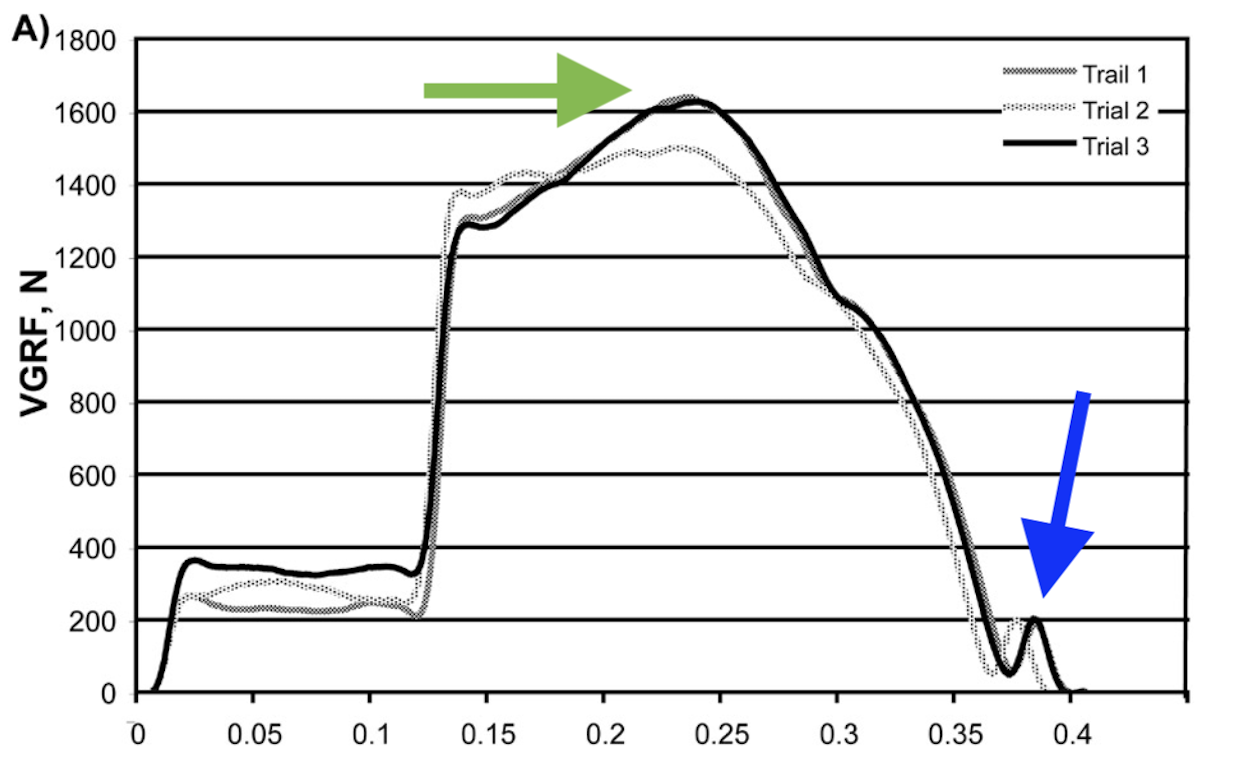
\includegraphics[width=0.25\textwidth]{figure/GRF1.png}}
\subfloat[Horizontal ground reaction force]{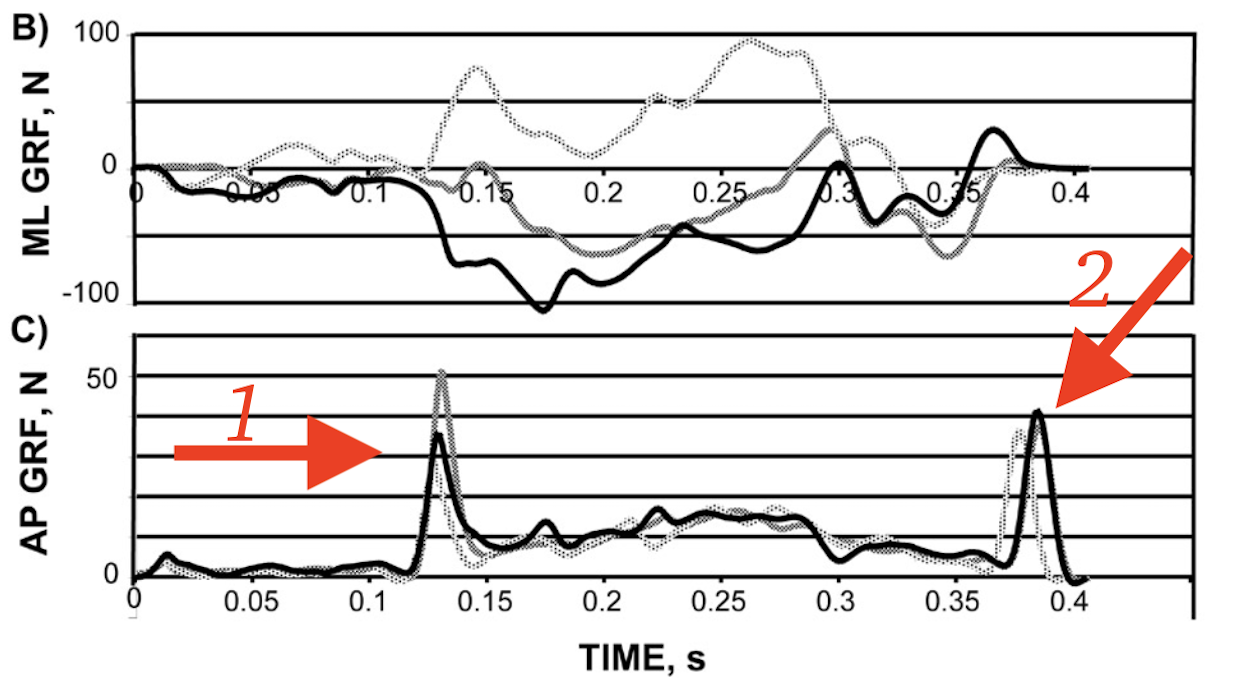
\includegraphics[width=0.25\textwidth]{figure/GRF2.png}}
\caption[Ollie ground reaction force]{Take-off ground reaction forces of the ollie. The green arrow is the highest peak, the blue arrow is the skateboard hitting the ground, the red arrows are friction peaks due to a hard push and tail impact respectively\cite{frederick_biomechanics_2006}}
\label{f_GRF}
\end{figure}
%%%%%%%%%%%%%%%% end figure %%%%%%%%%%%%%%%%%%%

\begin{figure*}[t]
\captionsetup[subfigure]{labelformat=empty}
    \subfloat[$t_1$=0.013]{{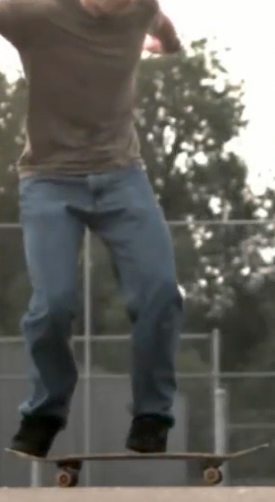
\includegraphics[width=0.13\textwidth]{figure/1.png} }}%
    \subfloat[$t_2$=0.129]{{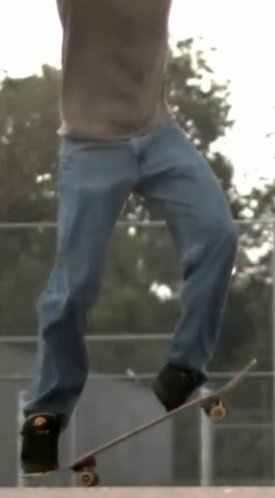
\includegraphics[width=0.13\textwidth]{figure/2.png} }}%
    \subfloat[$t_3$=0.181]{{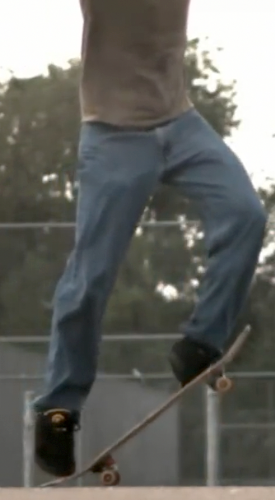
\includegraphics[width=0.13\textwidth]{figure/3.png} }}%
    \subfloat[$t_4$=0.187]{{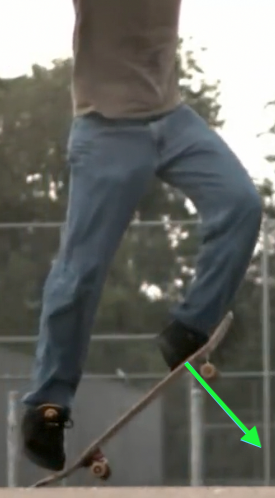
\includegraphics[width=0.13\textwidth]{figure/4.png} }}%
    \subfloat[$t_5$=0.303]{{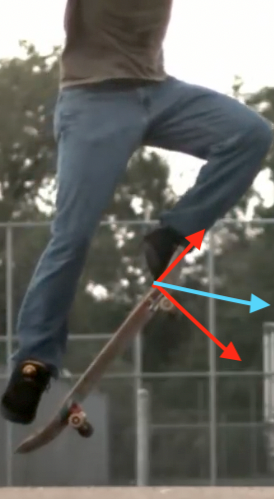
\includegraphics[width=0.13\textwidth]{figure/5.png} }}%
    \subfloat[$t_6$=0.431]{{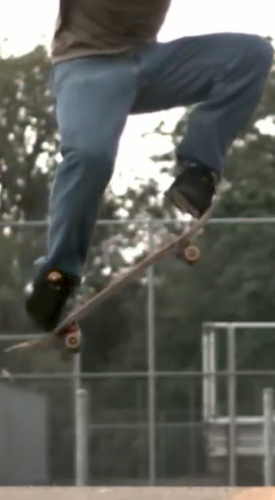
\includegraphics[width=0.13\textwidth]{figure/6.png} }}%
    \subfloat[$t_7$=0.543]{{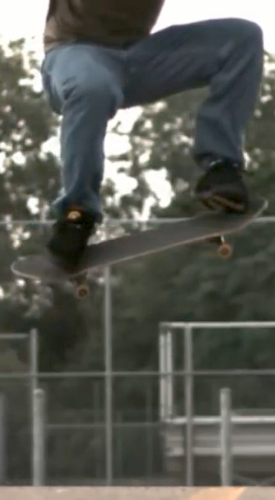
\includegraphics[width=0.13\textwidth]{figure/7.png} }}%
    \protect\newline
    \centering
    \subfloat[$t_8$=0.676$^1$]{{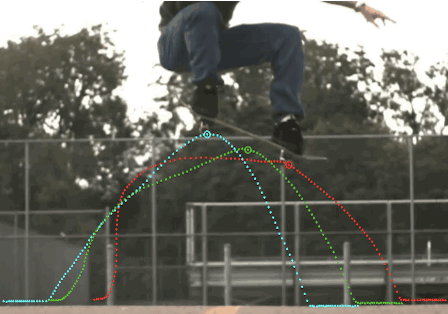
\includegraphics[width=0.336\textwidth]{figure/ollie_tracking_mid.png} }}
    \subfloat[$t_9$=0.722]{{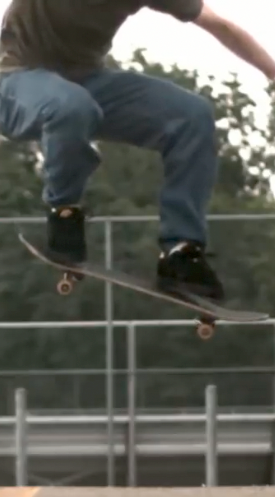
\includegraphics[width=0.13\textwidth]{figure/9.png} }}%
    \subfloat[$t_{10}$=0.904]{{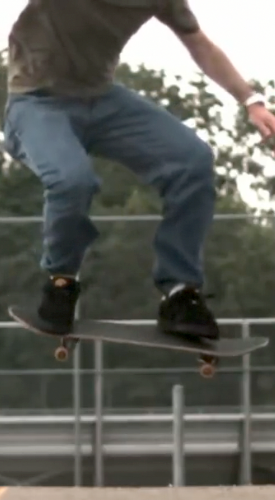
\includegraphics[width=0.13\textwidth]{figure/10.png} }}%
    \subfloat[$t_{11}$=1.097]{{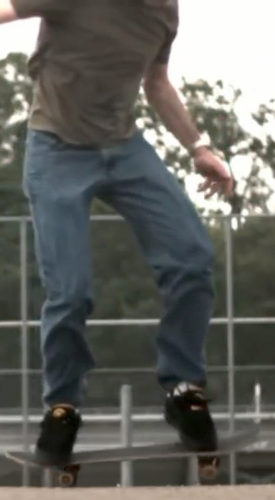
\includegraphics[width=0.13\textwidth]{figure/11.png} }}%
    \captionsetup{singlelinecheck=off}
    
    \vspace{-0.2cm}\caption[Ollie motion cues]{Green arrow: resultant force without friction, red arrows: force components whith friction, blue arrow: resultant force with friction. Blue-, green- and red line are trajectory of back wheel, middle and front wheel respectively\footnotesize\begin{itemize}
    \item[$t_1$] The skater is pushing firmly from his back leg and is starting to have less force on the front foot which results in the wheel just leaving the ground.
    \item[$t_2$] The front foot starts sliding relative to the board for the first time.
    \item[$t_3$] Tail collides with the ground, the front foot is still sliding and the back foot is barely in contact with the skateboard. 
    \item[$t_4$] Back foot is no longer in contact with the skateboard, the back wheels are not in contact with the ground anymore.
    \item[$t_5$] The front foot reached the nose of the skateboard.
    \item[$t_6$] Back foot contacts the board again.
    \item[$t_7$] Board is leveled out by the front foot.
    \item[$t_8$] Highest point is reached. Knees are fully tucked in. Feet are firmly placed on the deck. 
    \item[$t_9$] Front foot loses contact.
    \item[$t_{10}$] Board is horizontal, both feet are in contact.
    \item[$t_{11}$] The back wheels touch the ground and legs are almost fully streched out.
    \item[$^1$] \url{https://www.wired.com/2014/10/skateboard-physics-empzeal}
    \item[$^2$] \url{https://www.youtube.com/watch?v=339k4XEvbxY}
\end{itemize}}
    \label{f_olliesteps}
\end{figure*}

\noindent To understand the mechanics of the ollie, I analyzed a video to find motion cues during the ollie. The video was shot with a Redlake N3 high speed camera at 1000 fps and played back at 60 fps, the time of the events is calculated by taking the time in the video-editor and multiplying it by 1000/60. In a video editor the exact times are noted and a screenshot is taken whenever a distinct motion cue was observed. These motion cues ($t_1-t_{11}$) are given in figure \ref{f_olliesteps}. 

From the video it is clear that both feet can be in contact or not in contact with the board. The collision of the tail with the ground is only applied to the skateboard. The athlete is barely in contact with the skateboard and has already jumped when impact occurs. This is not interpreted in the findings of Fredericks et al. \cite{frederick_biomechanics_2006}. It is stated that the ground reaction force is typically described by a high magnitude peak due to the back foot pushing to the tail and slamming the tail into the ground (see figure \ref{f_GRF} green arrow). Though, after the large peak there is a tiny peak (blue arrow). This peak corresponds to the skateboard hitting the ground. The centre of mass (COM) of the human is already moving upwards and only the skateboard collides with the ground, not the skater. This same tiny peak is found when performing a kick-flip, a similar movement to the ollie but with a rotation about the x-axis(see figure \ref{f_skateterminology} for convention) \cite{determan_kinetics_2006}. 

This is confirmed in a paper by Nakashima \cite{nakashima_simulation_2021} stating that both feet should separate from the deck before the tail of the deck hits the ground. He also stated that the rotational velocity is mostly responsible for the skateboards' upward motion. When creating enough momentum about the rear axle, the rotational speed will provide an upward acceleration. 

The frictional forces seen in figure \ref{f_GRF} (red arrows) also suggest that the small peak is due to the impact of the skateboard. The ollie during the ground reaction force of figure \ref{f_GRF} was performed with a horizontal velocity resulting in a frictional contact of the tail scraping on the ground. When the tail hits the ground, friction should increase on the force plate. The only moment that friction increases is when a hard downward push creates an increase in rolling resistance (red arrow 1), and when the tail hits the ground (red arrow 2). The force is already below 200 [N] at that time instance, meaning that the human is either already airborne or about to be airborne.

Friction is not only seen during the impact, but also between the feet and the griptape. Due to the normal force perpendicular to the board together with a friction force tangential to the surface, the resultant force will take the form of a similar nature as shown in figure \ref{f_olliesteps}, $t_5$. If no friction would be present during this contact the resultant force would point more down as shown in $t_4$, resulting in a lower ollie. The higher the coefficient of friction between the foot and the deck, the more up the resultant force will be. And lastly it can be concluded that the bio mechanical obstruction of the feet cause the skateboard to not go further up. The knees are fully tucked in at the highest point, the skateboard can't go higher through this physical bound. 

A real skateboard bends and flexes during the ollie, but I decide to assume an rigid body model of the skateboard because of the increased complexity. Also, bending is a source of energy dissipation in addition to the energy loss due to local deformation \cite{stronge_impact_2000}. This suggests that an infinitely stiff board would dissipate the least energy, which would result in the highest ollies. On the other hand flexure of the board could serve as an energy storage for the human that could not have been used otherwise. For example in snowboarding, the flexure is used to gain upward momentum. In this paper flexure is not taken into account and could be an interesting topic for future researchers.

